\documentclass[11pt]{article}
\usepackage[a4paper,margin=1in]{geometry}
\usepackage{array}
\usepackage{booktabs}
\usepackage{graphicx}
\usepackage{longtable}
\usepackage{natbib}
\usepackage{xurl}
\usepackage[hidelinks]{hyperref}
\setlength{\parskip}{0.65em}
\setlength{\parindent}{0pt}
\emergencystretch=3em

\title{Relaytic-AML: Claim-Gated Evaluation Environments for Temporal Graph Financial-Crime ML}
\author{Author Name\\Affiliation\\\texttt{contact@example.com}}
\date{June 2026}

\begin{document}
\maketitle


\begin{abstract}

Relaytic-AML is a local-first inference-engineering environment for financial-crime machine learning. Its central claim is architectural: serious AML work needs a controlled local lab where data posture, mandate, specialist-agent roles, search budgets, model evidence, operational review assumptions, and public claim boundaries are all explicit artifacts. The system treats local disk artifacts as the source of truth; optional LLM or external-agent help consumes redacted, rowless context by default and cannot override deterministic gates. Specialist roles inspect source contracts, challenge modeling plans, execute bounded searches, materialize evidence cells, and govern what can be said publicly. Benchmarks are therefore used as probes of the architecture rather than as the identity of the system. In the current release pack, PaySim and Elliptic rows provide supporting evidence only, including a PaySim competitive test PR-AUC 0.638773 and an Elliptic temporal graph-feature test PR-AUC 0.668756. Elliptic2 remains modern context only: the local repeated official-partition candidate reports PR-AUC 0.94324 +/- 0.000882, below the recorded RevClassifyDS reference of 0.974, and reference-protocol plus cohort gates remain unresolved. The contribution is a reproducible, agent-usable, local-first AML evaluation environment that prevents benchmark scores, operational estimates, limitations, and public claims from drifting apart.

\end{abstract}

\section{Introduction}

AML systems are operational decision systems, not just classifiers. Investigators need temporally valid predictions, graph or entity provenance, a calibrated review queue, and defensible statements about what the evidence does and does not prove. They also need a way to run this work where sensitive data, intermediate artifacts, and decision rationales remain under local control.

Relaytic-AML starts from that product and research need. It is a local-first inference lab built around capability-scoped specialist roles rather than a single opaque agent or a single model family. A human operator can ask where the project stands, what artifacts matter, and which actions are safe next. An external coding agent or LLM can receive a redacted context pack and continue work without guessing hidden state. The system remains usable without any LLM because the canonical state is deterministic JSON, Markdown, TeX, and model artifacts on local disk.

Benchmarks still matter, but they are not the center of the thesis. They are stress tests for whether the local lab can keep source posture, split rules, model-search budgets, leakage posture, operating points, review-budget estimates, figure provenance, public-claim gates, and source-release audits aligned. A result that is useful on one benchmark can be misleading if it is promoted as a broader real-world AML claim; Relaytic-AML makes that promotion decision explicit and auditable.

\section{Contributions}

This paper makes seven contributions.

\begin{enumerate}
\item A local-first architecture for AML inference work where local artifacts remain canonical and optional LLM or external-agent help is advisory, redacted by default, and gate-constrained.
\item A role model for specialist agents: source/task scouts, guide and assist surfaces, scientist/challenger agents, builders, search controllers, claim governors, release governors, and external-agent handoff surfaces.
\item An evidence-cell contract for AML evidence rows that binds each reported number to dataset, split, command, artifact field, budget tier, leakage posture, operating-point policy, and claim state.
\item A deterministic claim-gate layer that separates supporting evidence from blocked or headline-eligible claims before paper text and public wording are generated.
\item A budget ladder that distinguishes smoke, baseline, competitive, and release runs so weak first-pass rows cannot be laundered into strong claims.
\item A release-safety pipeline that blocks public wording when clean-clone, claim-lint, leak-scan, citation, figure, or publishability gates fail.
\item A transparent first evidence pack over PaySim, Elliptic, and Elliptic2-context tracks that demonstrates the architecture while preserving limitations instead of converting proxy or blocked evidence into broader claims.
\end{enumerate}


\section{Research Questions}

The paper evaluates three systems questions.

\begin{enumerate}
\item Can a local-first AML lab make source posture, agent roles, model evidence, operational assumptions, and public claims inspectable from one artifact graph?
\item Can humans and external agents understand where a Relaytic run stands, what options are safe, and what evidence is missing without reading raw logs or private data?
\item Can claim gates prevent supporting proxy, graph-feature, and modern-context evidence from becoming unsupported hard AML or benchmark-superiority claims?
\end{enumerate}


\section{Local-First Agent Architecture}

Relaytic is designed around a simple control rule: the user's workspace is the authority. Raw and licensed data remain local by default; run directories, manifests, traces, metric cells, and release artifacts are the durable record; semantic caches, memory indexes, and LLM summaries are derived views. This is the opposite of a remote-first agent that sends private rows to a hosted planner and later reconstructs provenance from a conversation transcript.

The system is agentic, but the agents are not free-floating personalities. They are capability-scoped roles with bounded read/write surfaces, explicit budgets, and artifact obligations. A Scout can inspect source posture and split risk. A Scientist can challenge baselines or propose ablations. A Builder can execute a controlled run. A claim governor can reject public wording even when the model score looks attractive. A guide or assist surface can explain the state to a human or export a redacted context pack to another LLM.

\begingroup
\small
\setlength{\tabcolsep}{3pt}
\begin{longtable}{>{\raggedright\arraybackslash}p{0.21\linewidth} >{\raggedright\arraybackslash}p{0.21\linewidth} >{\raggedright\arraybackslash}p{0.21\linewidth} >{\raggedright\arraybackslash}p{0.21\linewidth}}
\toprule
Role & What it owns & Local-first boundary & Main artifacts \\
\midrule
\endfirsthead
\toprule
Role & What it owns & Local-first boundary & Main artifacts \\
\midrule
\endhead
Operator and mandate owner & Sets goals, constraints, privacy posture, and stop/continue preferences. & Can keep all data on a controlled local machine, server, or cluster. & Mandate, policy, permission, and next-action artifacts. \\
Guide and assist layer & Answers where the run is, what artifacts matter, and which action is safe next. & Uses local artifacts first; optional LLM help is advisory and redacted by default. & Guide payloads, assist turns, status, and context packs. \\
Scout and task-contract agents & Inspect source posture, target semantics, split validity, and leakage risk. & Work from staged local snapshots rather than mutating the original data source. & Dataset registry, source manifests, split contracts, and task reports. \\
Scientist and challenger agents & Propose baselines, ablations, shadow candidates, and failure explanations. & Candidate work is bounded by explicit budgets and local artifact permissions. & Experiment registry, scorecards, ablations, and shadow-trial reports. \\
Builder and search controller & Execute reproducible model/search plans and select thresholds on validation evidence. & Optional adapters are versioned and never become hidden sources of truth. & Run directories, model artifacts, search traces, and operating-point records. \\
Claim and release governors & Decide which evidence can be said publicly and which claims stay blocked. & Fail closed on leakage, missing provenance, unsafe wording, or dirty release state. & Metric cells, claim lint, release manifests, and arXiv source audits. \\
External agents or LLMs & Consume exported context, propose repairs, or continue work through stable surfaces. & Receive rowless/redacted context unless policy explicitly grants richer access. & External context packs, handoff reports, and reproducible commands. \\
\bottomrule
\end{longtable}
\endgroup


Two design choices are load-bearing. First, all important work produces a local artifact that another human or agent can inspect. Second, every optional intelligence path is subordinate to that artifact graph. A local LLM may help phrase guidance, and a frontier model may help propose repairs, but neither becomes the source of truth unless its proposal is converted into a reproducible local artifact and passes the same gates.

\begin{figure}[htbp]
\centering
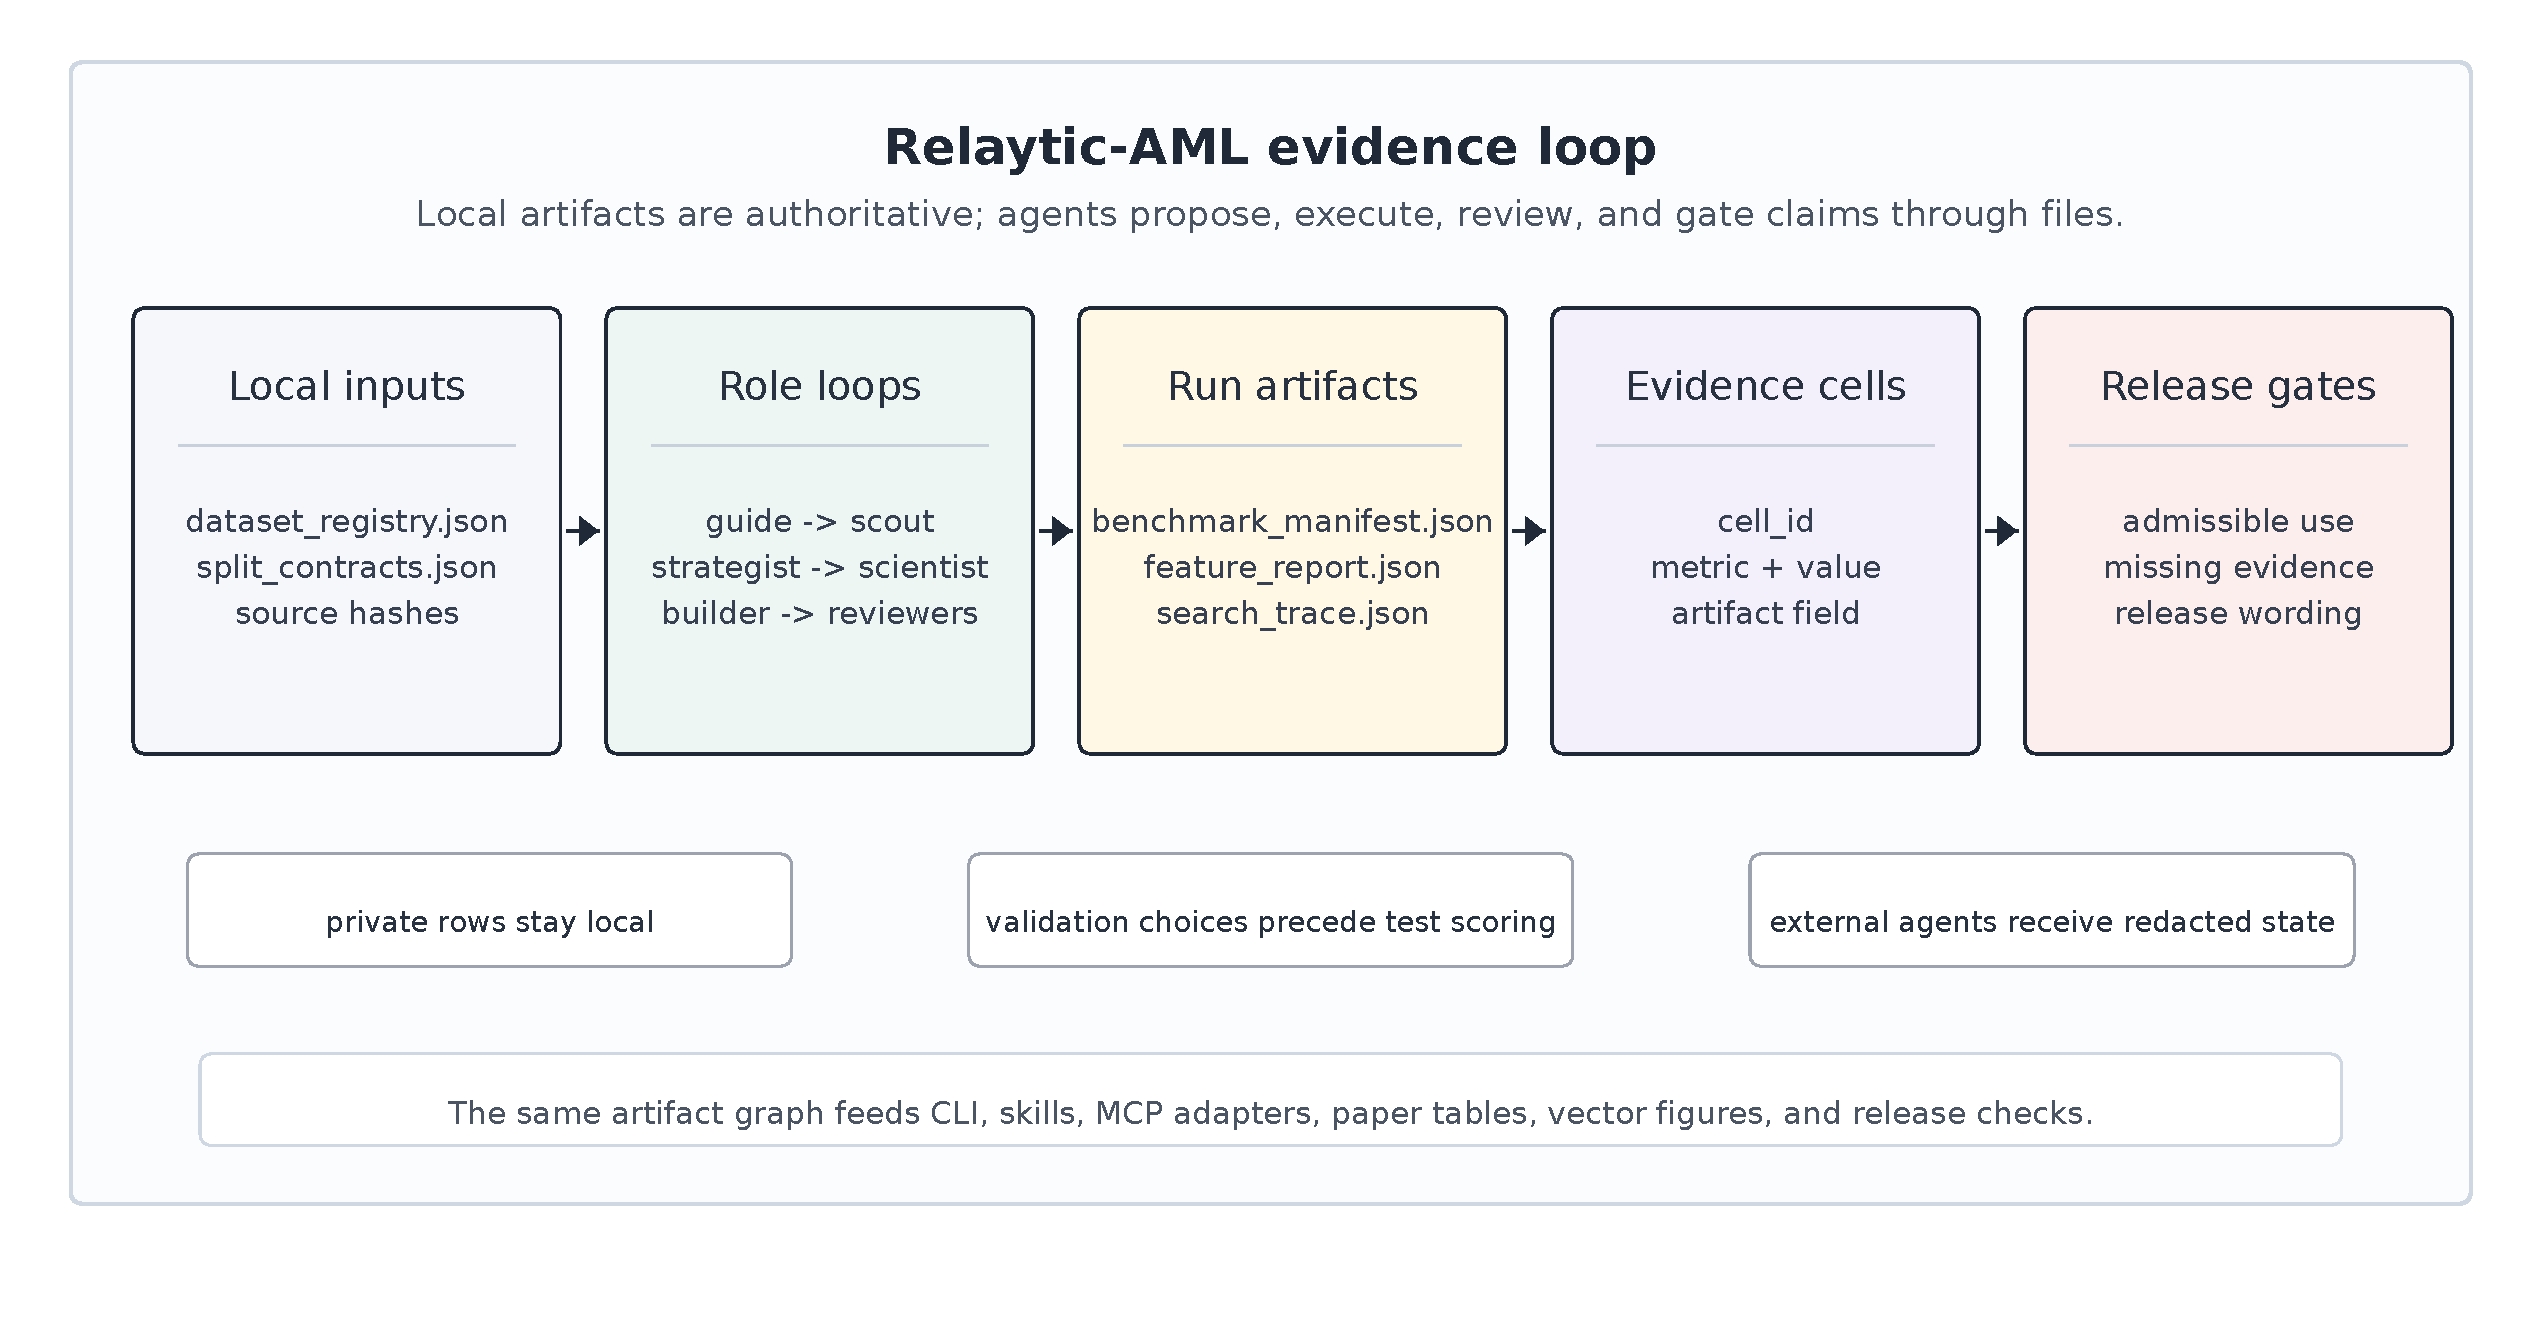
\includegraphics[width=0.94\linewidth]{figures/figure_1_claim_gate_flow.pdf}
\caption{Local-first Relaytic agent architecture}
\end{figure}

\section{Current Frontier Context}

The current AML frontier is not one single leaderboard. It is a set of pressure points that make evaluation harder: real graph scale, realistic entity behavior, temporal drift, operational throughput, and scientifically reliable agent-generated experiments. Relaytic-AML is designed as infrastructure around those pressure points rather than as a replacement for detector papers.

PaySim is a synthetic mobile-money simulator designed to address the scarcity of legitimate public mobile-transaction datasets for fraud research \cite{lopezrojas2016paysim}. It is useful for temporal transaction-fraud workflow evaluation, but synthetic evidence cannot by itself establish hard real-bank AML performance.

The Elliptic Bitcoin dataset introduced a public transaction graph with more than 200K transaction nodes, 234K directed payment-flow edges, and 166 node features across 49 time steps \cite{weber2019elliptic}. That work also showed why graph evidence must be compared against strong simpler baselines rather than assumed superior.

Elliptic2 shifts the public AML benchmark center toward subgraph learning, with 121,810 labeled subgraphs inside a background graph of roughly 49M node clusters and 196M edge transactions \cite{bellei2024elliptic2}. RevTrack and RevClassify further argue that sender and receiver context around a subgraph can be a powerful and scalable signal \cite{song2024revtrack}. These works motivate Relaytic-AML's modern-context and limitation track, but they do not make the current Relaytic Elliptic2 row a performance contribution.

The 2025/2026 AML graph literature also raises the bar beyond the current Relaytic evidence rows. TransXion frames benchmark realism around profile-aware simulation, rich entity attributes, non-template illicit synthesis, and out-of-character behavior \cite{chen2026transxion}. LineMVGNN and ExSTraQt represent detector-focused work on directed money flow, edge-aware graph views, and quasi-temporal transaction representations \cite{poon2026linemvgnn,tariq2026extraqt}. BlazingAML stresses throughput and fuzzy multi-stage scheme expression as a systems problem \cite{ye2026blazingaml}, while continual graph-learning reviews emphasize drift, adaptation, class imbalance, and evolving laundering behavior \cite{deprez2025continualaml}. Relaytic-AML is positioned as complementary infrastructure for such work: it does not claim detector parity with these systems, but it makes dataset posture, split validity, budgets, limitations, and public claims auditable.

The paper also follows broader ML documentation and reproducibility practice. Datasheets for Datasets and Model Cards argue for explicit dataset and model reporting \cite{gebru2021datasheets,mitchell2019modelcards}. The NeurIPS reproducibility program highlights the need for code, data, and checklist discipline in ML research \cite{pineau2021reproducibility}. Recent work on ML research agents warns that coherent papers can still contain invalidated experiments, reinforcing the need for executable artifacts and claim gates \cite{chen2025mlrbench}.

\section{Methodology: Evidence Cells, Gates, and Budgets}

Relaytic-AML treats a paper metric as an evidence cell, not as a free-standing score. An evidence cell is a tuple consisting of dataset identity, split contract, execution command, run-directory or artifact reference, artifact field, metric value, budget tier, leakage posture, operating-point rule, claim state, and gate limitation notes. The table generator reads only these cells, and the paper generator cites the cell identifier for every numeric row.

A claim gate is a deterministic predicate over evidence cells and release artifacts. In this release, the gate can assign a row to supporting-only evidence, modern-context-only evidence, baseline-only evidence, or blocked evidence. No row is headline-eligible. The same gate also lints generated paper text and public wording, so unsupported phrases such as hard AML superiority, claimed equivalence to RevClassify, graph-neural superiority, hard business value, or leaderboard-winner claims remain blocked.

The method has three layers. First, evidence cells make every number traceable. Second, claim gates decide what the number is allowed to mean. Third, release gates decide whether the public package is coherent enough for outside review. This is intentionally conservative. It is designed for settings where a strong-looking model number can be less important than the question of whether the number was produced under a valid split, compared against an appropriate baseline, selected without test leakage, and described with the right scope.

Budgeting is part of the method rather than an afterthought. Smoke budgets test that commands and artifact contracts exist. Baseline budgets provide conservative full-dataset rows. Competitive budgets add stronger feature families, validation-only operating-point selection, calibration, and model search. Release budgets freeze the transformation from benchmark artifact to paper table, figure, public wording, and source bundle. A weak smoke result can therefore inform debugging without becoming a paper claim.

\section{Evidence Operating Layer}

The local-first architecture becomes concrete through an evidence operating layer. In this paper, Relaytic-AML is the financial-crime edition of that system. It is not only a model runner; it coordinates source posture, task semantics, split discipline, model search, decision thresholds, review queues, artifacts, and public claim boundaries.

The architecture has six cooperating layers.

\begin{enumerate}
\item Source and task contracts: dataset registries, access posture, target semantics, benchmark-vs-deployment separation, and split contracts.
\item Execution and search: benchmark runners, adapter eligibility, budget profiles, model-family search, calibration, threshold selection, and optional shadow candidates.
\item AML domain layer: graph/entity extraction, typology posture, suspicious-subgraph scoring, review-queue metrics, delayed-label posture, and operational burden estimates.
\item Evidence ledger: metric cells, table provenance, figure provenance, limitation matrices, and reproduction commands.
\item Claim and release gates: claim lint, public wording guards, leak scans, clean-clone proof, arXiv-source audits, and package checklists.
\item Handoff surfaces: guide, assist, status, mission-control, and external-LLM context export so humans and agents can ask where the project stands and what action is safe next.
\end{enumerate}


This architecture makes the system useful even when a detector claim is blocked. A blocked row is not discarded; it becomes a structured research state with a reason, an artifact reference, and a repair path.

\section{Special Features and Intended Uses}

Relaytic-AML is intended for local evaluation labs where teams need to test claims before deployment, publication, or procurement. The most important features are not tied to a single model family.

\begin{enumerate}
\item Artifact-first reproducibility: generated tables and figures are derived from JSON artifacts rather than hand-written spreadsheet state.
\item Local-first privacy posture: private or licensed datasets stay outside the repository, while hashes, manifests, and access posture can still be audited.
\item Claim-gated communication: public text is linted against allowed and blocked claims, reducing the risk that benchmark evidence becomes marketing language.
\item Budget-aware model development: smoke, baseline, competitive, and release tiers separate engineering checks from serious benchmark evidence.
\item Operational evaluation: review-budget precision, recall, false-positive burden proxies, and case-packet completeness sit next to model metrics.
\item Agent-readable handoff: structured artifacts let external LLMs or coding agents inspect state, propose next experiments, and avoid unsupported assumptions.
\end{enumerate}


Companies can use Relaytic-AML to challenge incumbent rules or models on the same review queue, evaluate new datasets before committing analyst capacity, audit whether a vendor or internal model is being compared fairly, and prepare evidence packs for compliance or model-risk review. Researchers can use it as a controlled environment for asking whether an AML result is supported, blocked, or only useful as a limitation.

\section{Evaluation Environment}

Relaytic-AML is organized as a deterministic local evidence pipeline. Dataset registry artifacts define source and access posture. Split contracts define chronological, graph-snapshot, or subgraph partition rules. Benchmark runners produce model and operating-point artifacts. Paper-table generation consumes those artifacts and writes per-cell provenance. Draft, release, and arXiv-source generation then lint wording against publishability gates.

The environment has three design rules.

\begin{enumerate}
\item Local artifacts are the source of truth. Narrative text is derived from artifacts, not the reverse.
\item Validation selects models, thresholds, and operating points before fixed test evaluation.
\item Blocked evidence stays visible as a limitation, because hiding failed or incomplete tracks makes both human and agentic research less scientific.
\end{enumerate}


\section{Benchmark Protocol}

The benchmark protocol is deliberately subordinate to the architecture. Its purpose is to check whether Relaytic can produce traceable evidence, respect split and leakage contracts, expose operational assumptions, and block unsupported claims. It is not a claim that a single score defines the value of the system.

The current release pack separates smoke, baseline, competitive, and release budgets. Smoke checks prove that commands and artifacts exist. Baseline budgets establish conservative full-dataset evidence where possible. Competitive budgets use stronger features, candidate families, calibration, and validation-only operating-point selection. Release budgets freeze the paper transformation path and require clean-clone and leak-scan proof. A budget tier is part of the evidence cell, so the paper can distinguish a serious competitive run from a quick reproducibility check.

PaySim is treated as a synthetic temporal proxy. Elliptic is treated as temporal graph-feature supporting evidence. Elliptic2 is treated as modern subgraph context and limitation evidence, because the current local environment has not executed a faithful RevClassify reference-protocol match and the current-core to RevTrack-evaluable cohort boundary is not fully proven.

\begingroup
\small
\setlength{\tabcolsep}{3pt}
\begin{longtable}{>{\raggedright\arraybackslash}p{0.21\linewidth} >{\raggedright\arraybackslash}p{0.21\linewidth} >{\raggedright\arraybackslash}p{0.21\linewidth} >{\raggedright\arraybackslash}p{0.21\linewidth}}
\toprule
Evidence row & Metric & Value & Claim posture \\
\midrule
\endfirsthead
\toprule
Evidence row & Metric & Value & Claim posture \\
\midrule
\endhead
PaySim baseline & test PR-AUC & 0.331345 & baseline-only \\
PaySim competitive & test PR-AUC & 0.638773 & supporting-only synthetic temporal proxy \\
PaySim competitive & precision at review budget & 0.703336 & supporting-only \\
PaySim competitive & recall at review budget & 0.471584 & supporting-only \\
Elliptic graph-feature & test PR-AUC & 0.668756 & supporting-only graph-feature evidence \\
Elliptic graph-feature & precision at review budget & 1 & supporting-only \\
Elliptic graph-feature & recall at review budget & 0.056604 & supporting-only \\
Elliptic2 context & official-partition PR-AUC mean & 0.94324 & modern context only \\
Elliptic2 context & official-partition PR-AUC std & 0.000882 & modern context only \\
RevClassifyDS reference & published PR-AUC & 0.974 & reference context, not parity \\
\bottomrule
\end{longtable}
\endgroup


Exact metric-cell identifiers and artifact fields are stored in the metric-cell audit artifact named in the reproducibility section; none of these rows is a headline or hard AML claim.

\begin{figure}[htbp]
\centering
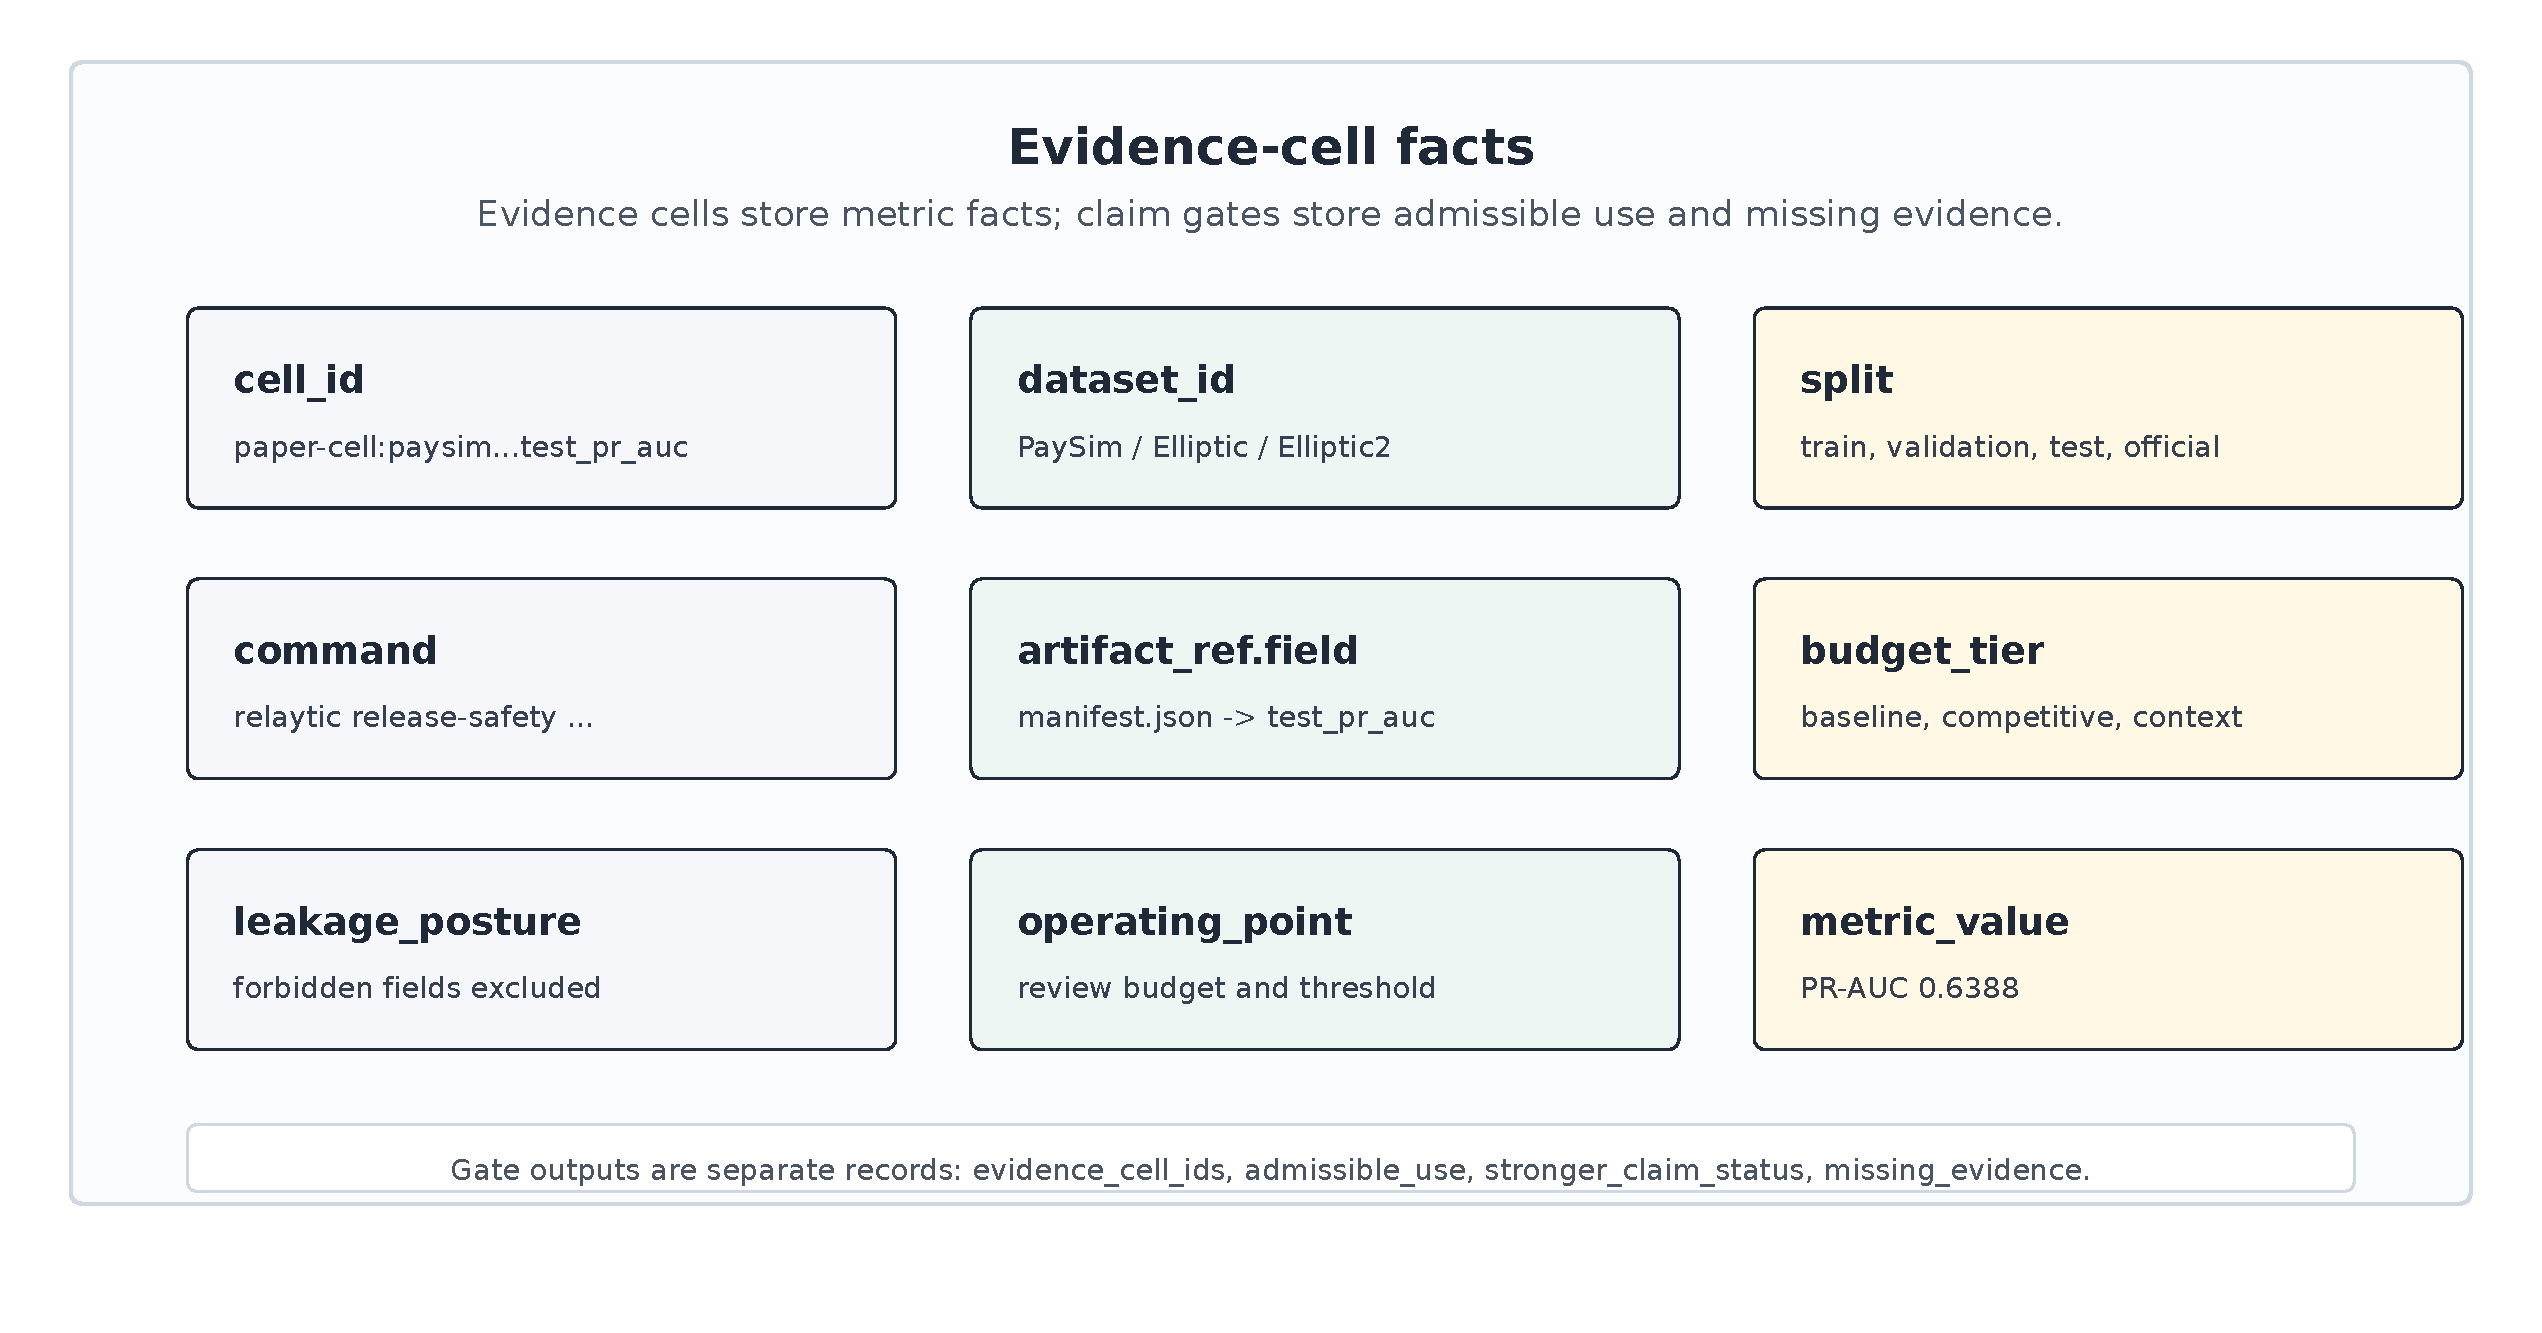
\includegraphics[width=0.94\linewidth]{figures/figure_2_supporting_pr_auc.pdf}
\caption{Supporting PR-AUC rows with claim posture}
\end{figure}

\begin{figure}[htbp]
\centering
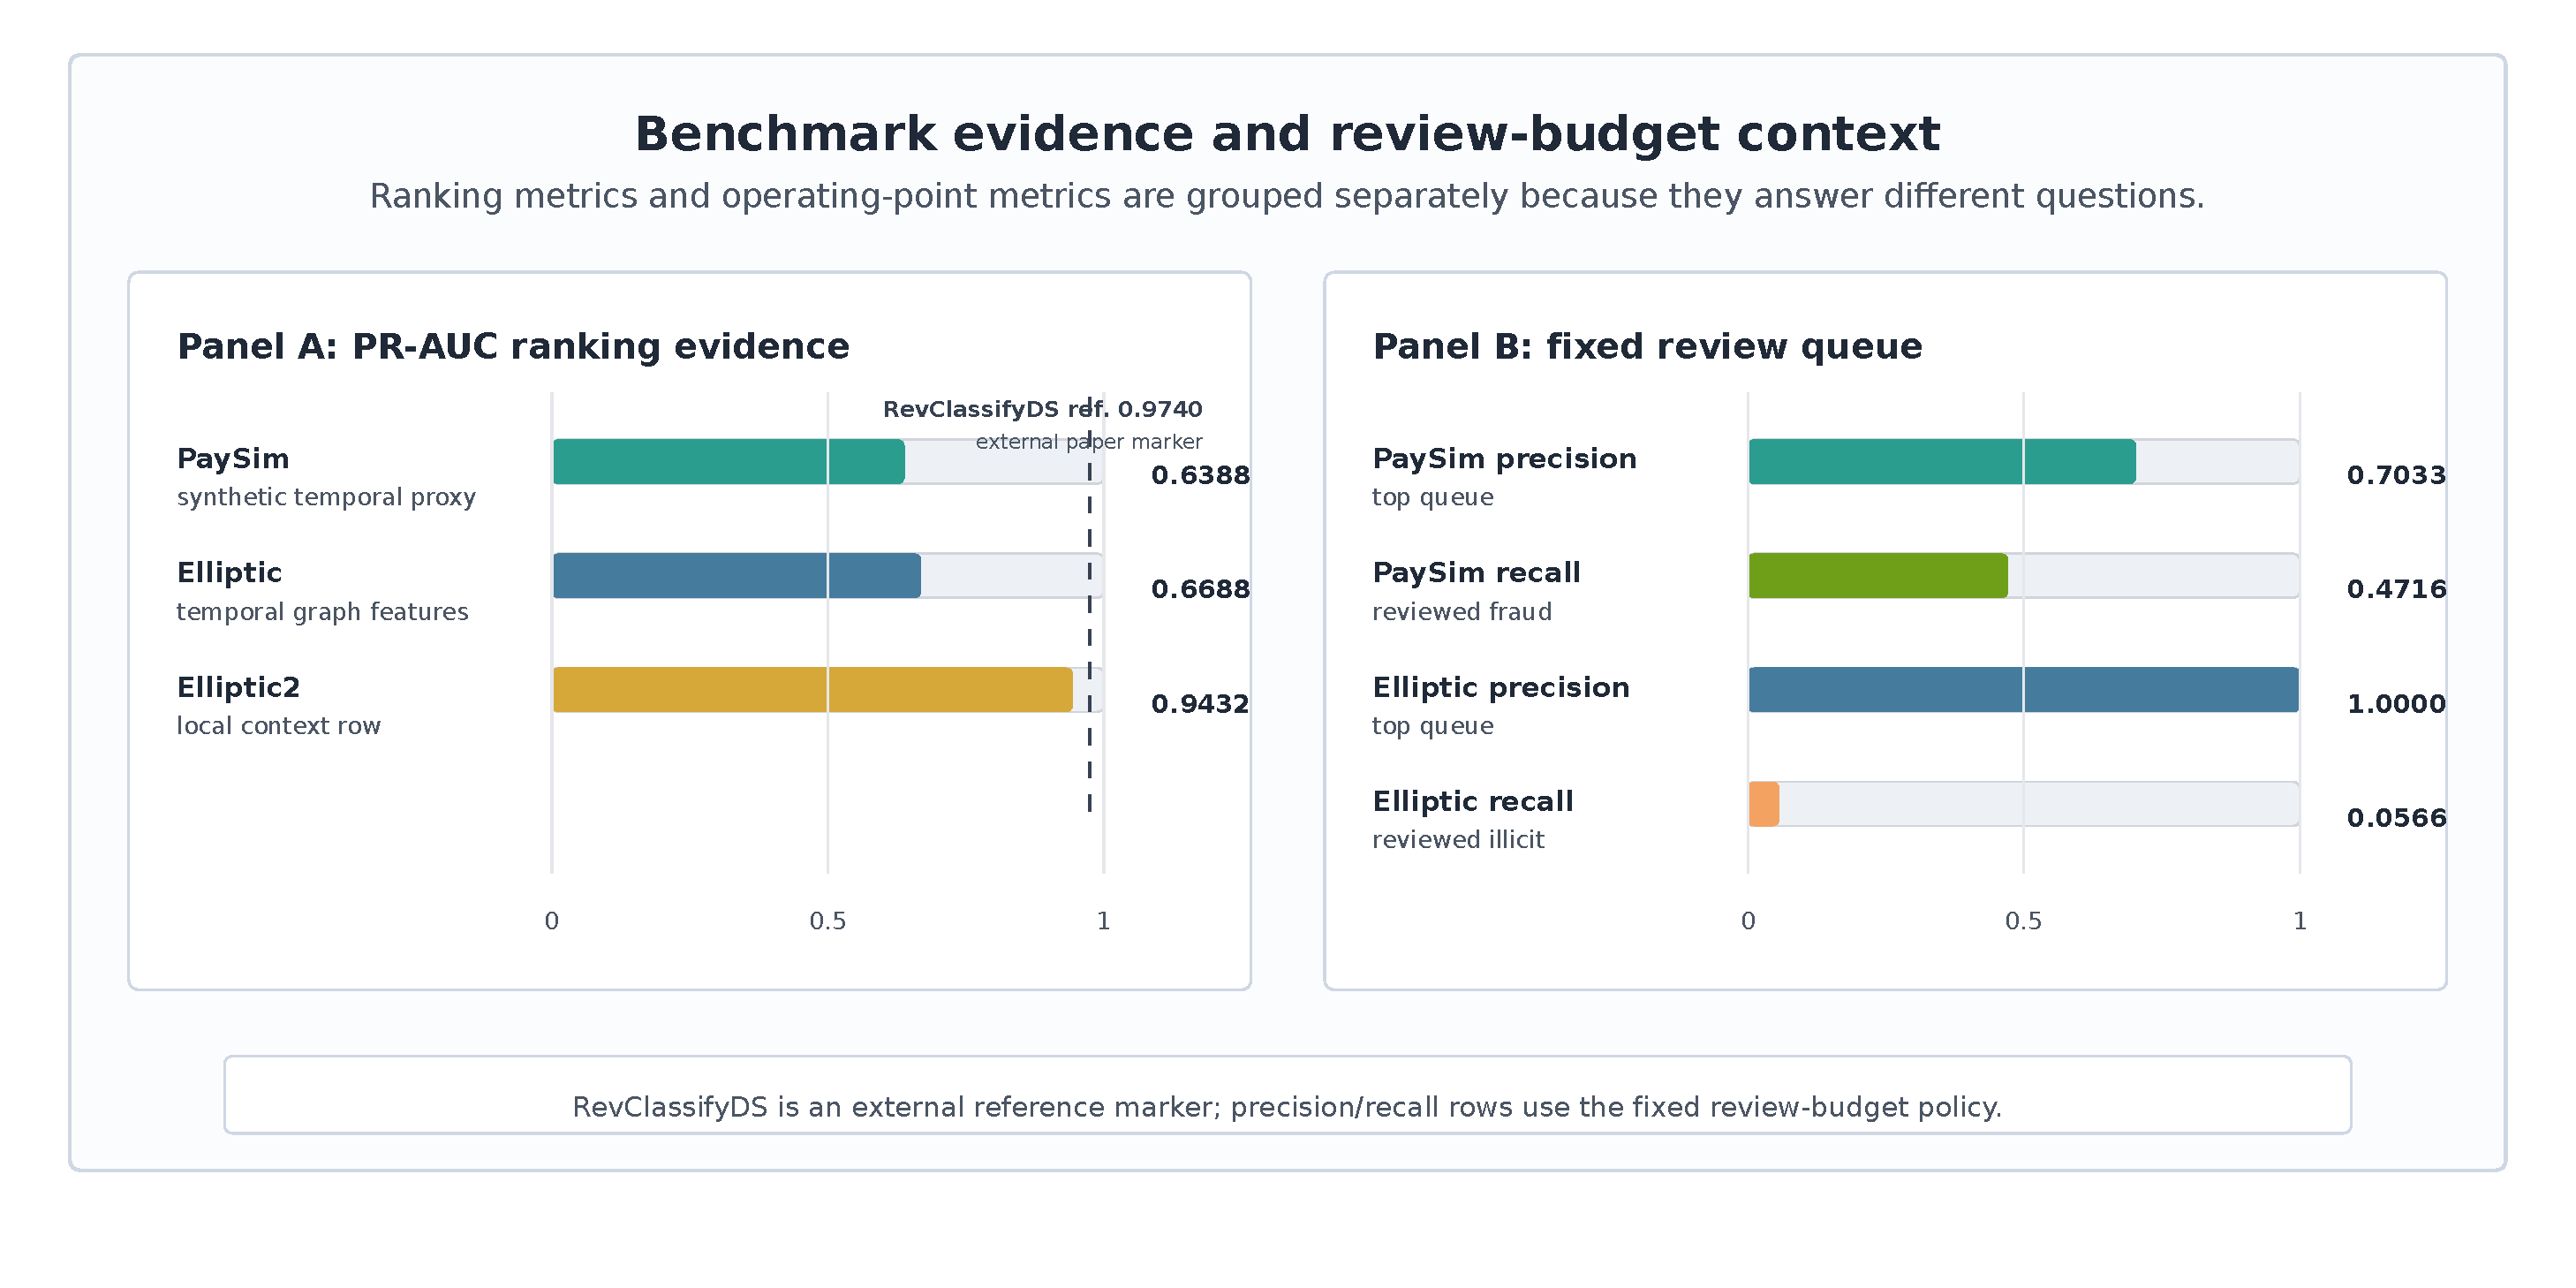
\includegraphics[width=0.94\linewidth]{figures/figure_3_review_budget.pdf}
\caption{Review-budget precision and recall}
\end{figure}

\begin{figure}[htbp]
\centering
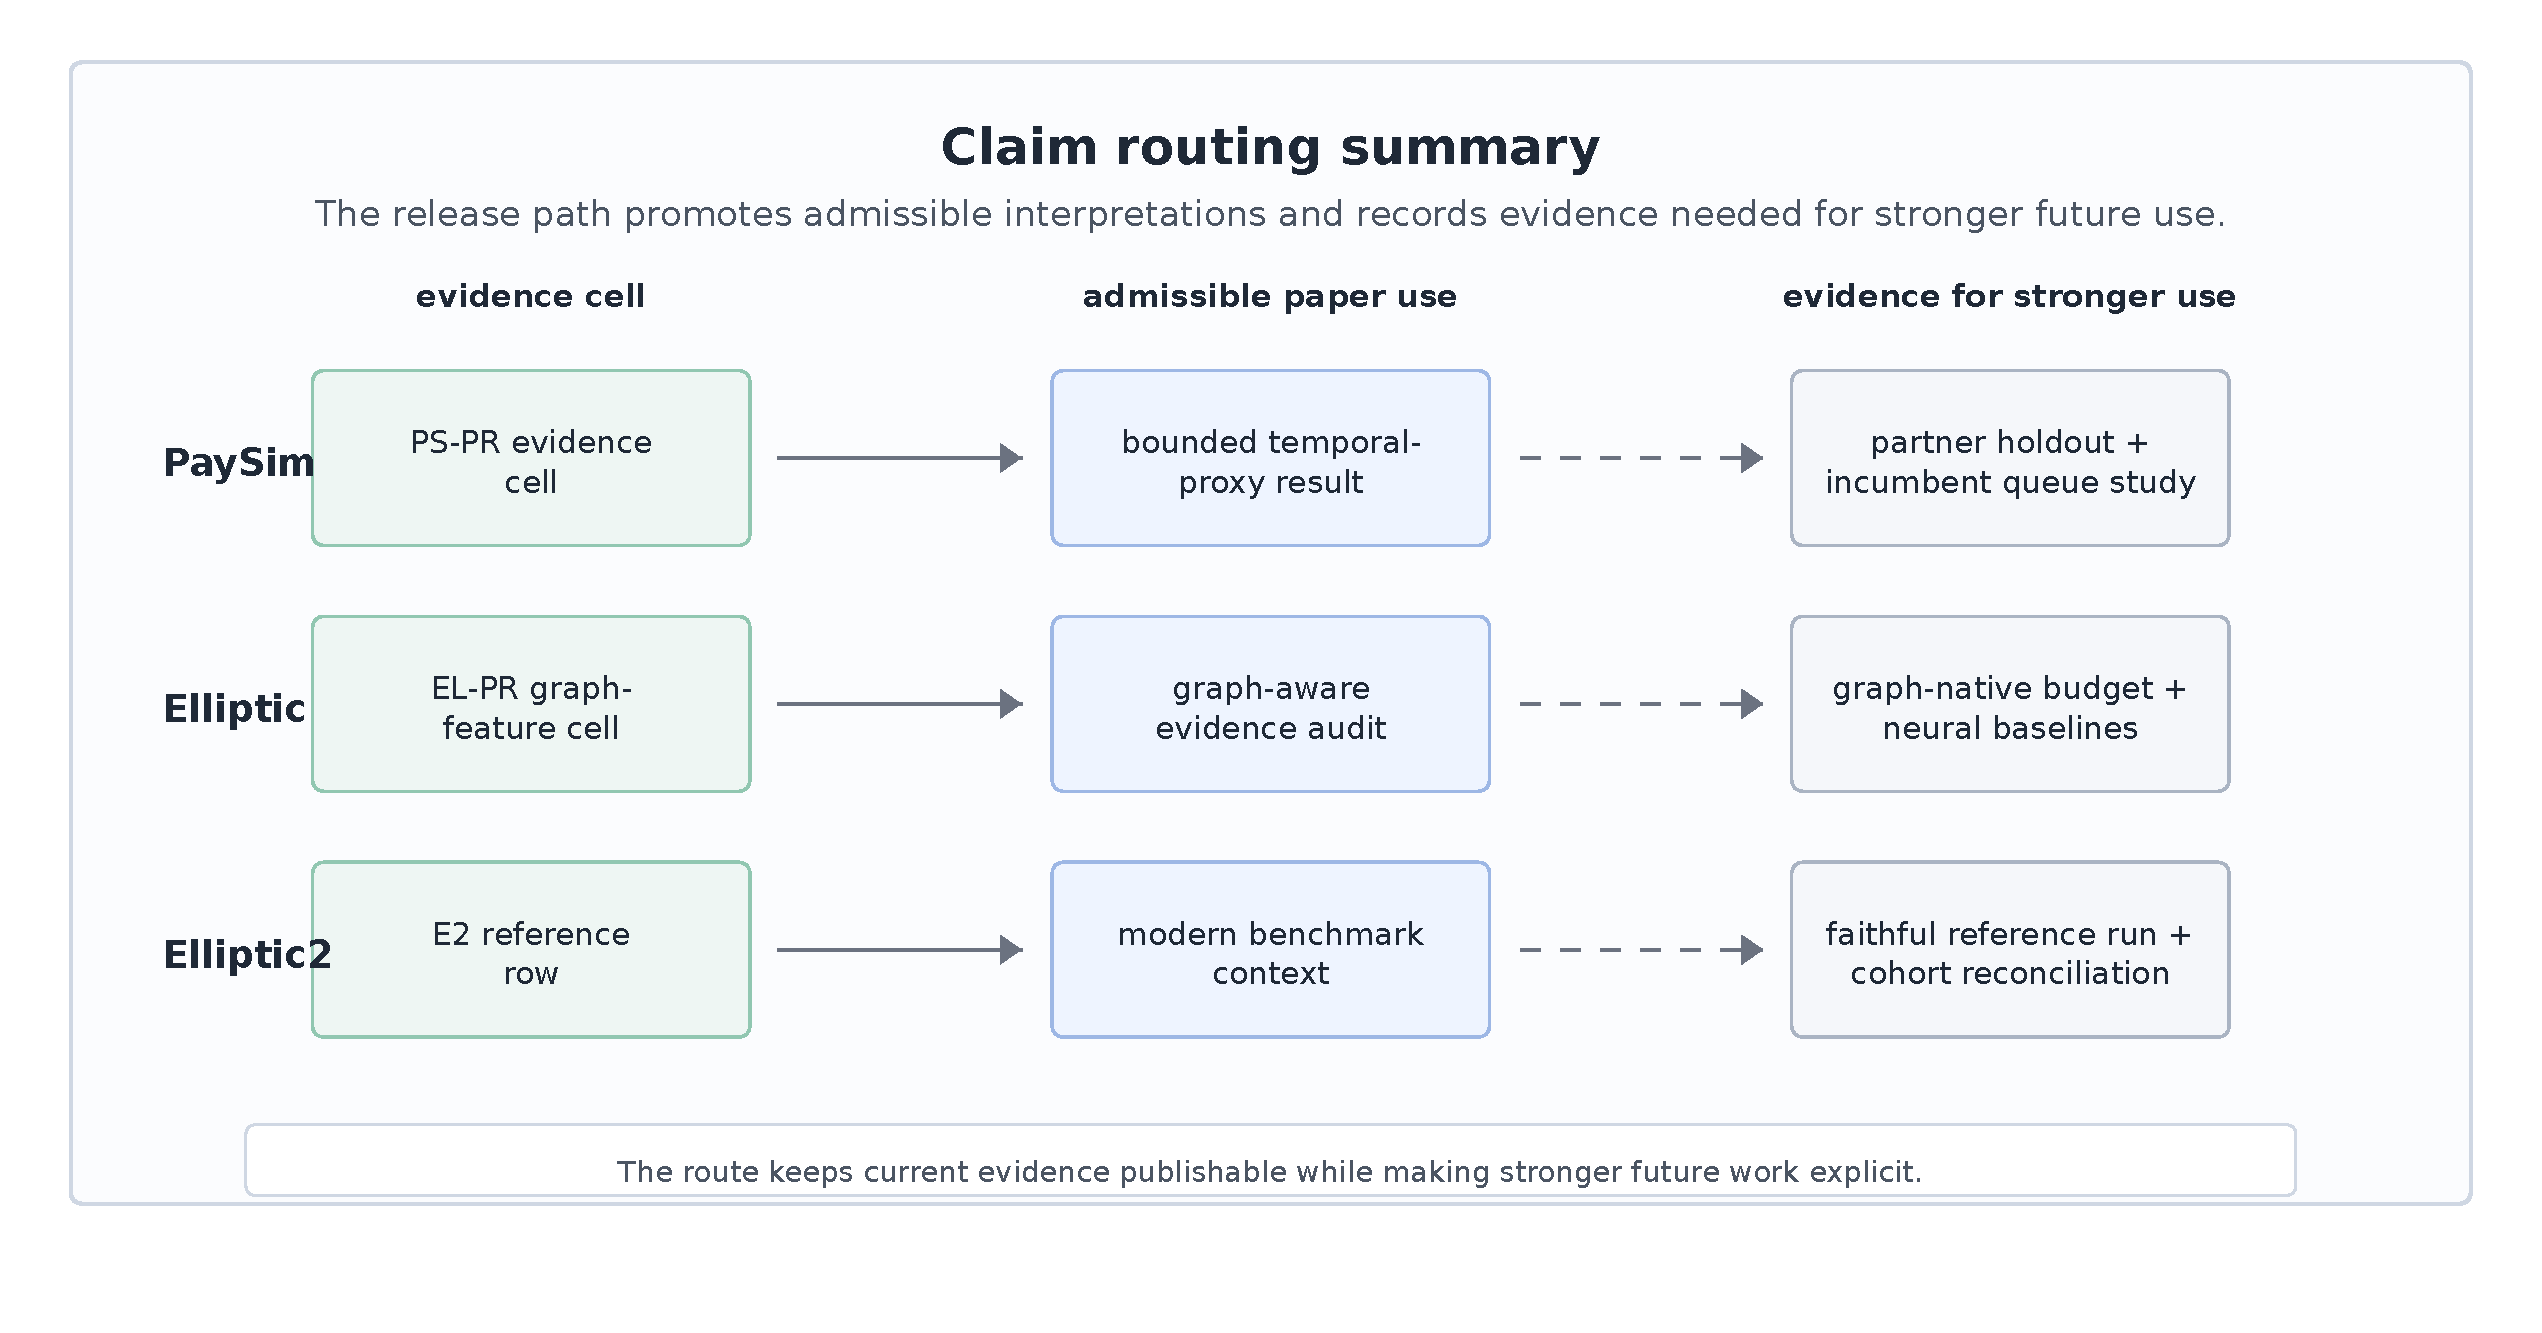
\includegraphics[width=0.94\linewidth]{figures/figure_4_publishability_matrix.pdf}
\caption{Claim boundaries and future unlocks}
\end{figure}

\section{Results}

The PaySim competitive row improves over the PaySim baseline inside the recorded synthetic temporal-fraud contract. The Elliptic graph-feature row is supporting graph evidence with modest structural lift, not graph-neural superiority. The Elliptic2 context row is strong enough to motivate future reprovisioning, but not enough to claim parity with the RevClassifyDS reference or to make an Elliptic2 performance contribution.

The most important result is the gate outcome: all current numeric rows are usable for a claim-safe evaluation-environment paper, and none is allowed to become a hard AML, production, benchmark-superiority, or business-value claim. That outcome is scientifically useful because it exposes what the environment knows and what it refuses to overstate.

\begingroup
\small
\setlength{\tabcolsep}{3pt}
\begin{longtable}{>{\raggedright\arraybackslash}p{0.17\linewidth} >{\raggedright\arraybackslash}p{0.17\linewidth} >{\raggedright\arraybackslash}p{0.17\linewidth} >{\raggedright\arraybackslash}p{0.17\linewidth} >{\raggedright\arraybackslash}p{0.17\linewidth}}
\toprule
Track & Current paper use & Blocked stronger claim & Evidence needed before promotion & Gate status \\
\midrule
\endfirsthead
\toprule
Track & Current paper use & Blocked stronger claim & Evidence needed before promotion & Gate status \\
\midrule
\endhead
PaySim temporal proxy & supporting synthetic temporal-fraud evidence & real-bank AML superiority & partner or real holdout with frozen release budget & supporting only \\
Elliptic graph-feature & supporting temporal graph-feature evidence & graph-neural or graph benchmark superiority & repeated graph release budget against strong feature baselines & supporting only \\
Elliptic2 subgraph & modern subgraph context and limitation evidence & Elliptic2 performance contribution or reference-method match & faithful RevClassify reproduction or leakage-resistant subgraph protocol & context only \\
Operational review layer & supporting review-budget estimates & hard analyst-hour or business-value claim & complete case packets and same-queue incumbent comparison & supporting only \\
\bottomrule
\end{longtable}
\endgroup


\section{Discussion}

The practical value of Relaytic-AML is not that it replaces a compliance platform or wins one benchmark table. Its value is that it can give risk, fraud, or AML teams a local evidence lab for unknown datasets, incumbent challenges, review-budget tradeoffs, leakage checks, and public-claim discipline. A company evaluating a new dataset can inspect whether the result is a model win, an environment win, a proxy-only result, or a blocked claim. That distinction is often what separates a useful internal experiment from an unsafe public or deployment claim.

For research teams and agentic ML workflows, the same structure is a guard against coherent but invalid experiments. External agents can consume the generated JSON artifacts, reproduce the paper tables, see blocked claims, and propose the next benchmark action without inferring hidden state from prose. The strongest story is therefore the artifact discipline: Relaytic-AML demonstrates that an ambitious evaluation system can still refuse claims it has not earned.

The system is also valuable when results are not spectacular. A low or blocked row can still tell a team that a dataset is synthetic-only, that a split leaks future information, that a graph-native candidate failed to beat strong tabular features, that a review-queue claim lacks a same-queue incumbent, or that a paper sentence is stronger than the evidence permits. In high-risk financial-crime settings, those negative answers are productive outputs.

\section{Limitations}

\begin{itemize}
\item \textbf{LIM-01-paysim-proxy}: PaySim is synthetic mobile-money fraud evidence. It is useful for a temporal proxy workflow, but it is not real-bank AML superiority evidence. Required repair: Add a real financial-crime holdout or partner-approved private evaluation before making hard AML claims.
\item \textbf{LIM-02-elliptic-supporting-graph}: The Elliptic row is a supporting temporal graph-feature result. It does not prove graph-neural or graph benchmark superiority. Required repair: Run repeated-seed graph baselines and promote a graph-native candidate only if it beats strong feature baselines under the same split.
\item \textbf{LIM-03-elliptic2-context-only}: Elliptic2 is retained as modern context and limitation evidence only; it is not a Relaytic performance contribution in this paper. Required repair: Reproduce the RevClassify reference setup faithfully or define a new leakage-resistant subgraph protocol with viable cohort proof.
\item \textbf{LIM-04-operational-assumptions}: Operational review-budget rows are supporting estimates because aggregate case packets, same-queue incumbent comparisons, and analyst-hour assumptions are not fully frozen. Required repair: Freeze case-packet completeness and compare against the same review queue or an approved incumbent baseline.
\item \textbf{LIM-05-clean-clone-smoke-scope}: P12 clean-clone and paper-smoke proof now passes for the generated paper path, including install-readiness checks, P10/P11 smoke regeneration, leak scan, and reproduction failure reporting. The remaining limitation is scope: heavy external-local benchmark reruns are documented but not rerun inside the P12 smoke proof. Required repair: run the heavy benchmark commands under a frozen release budget before promoting hard or headline benchmark claims.
\end{itemize}


Additional limitations remain. The current public evidence is not a deployment validation, does not include a bank-approved private holdout, does not reproduce the full RevClassify reference setup, does not prove analyst-hour savings against an incumbent queue, and does not yet include a true continual-learning benchmark row. The paper therefore focuses on evaluation discipline and source-package reproducibility rather than on a hard detector win.

\section{Future Work}

The next research steps are direct and measurable. The first group strengthens Relaytic as a local-first agentic lab; the second group expands benchmark and AML evidence.

\begin{enumerate}
\item Add role-level evaluations that test whether guide, scout, scientist, builder, claim-governor, and release-governor surfaces agree on the same local run state.
\item Expand redacted context-pack evaluation so external LLMs and coding agents can propose repairs while the claim firewall rejects unsupported paper edits.
\item Strengthen protocol-conformance proof across CLI, mission control, MCP-style hosts, source artifacts, and generated paper surfaces.
\item Add a real or partner-approved holdout track with frozen access posture, repeated-seed release budgets, and same-queue incumbent comparisons.
\item Reprovision Elliptic2 with a faithful RevClassify reference-protocol reproduction or define a leakage-resistant subgraph protocol with clear cohort proof.
\item Add a TransXion-style profile-aware simulation track so context-aware and out-of-character behavior can be evaluated under the same claim gates.
\item Add continual graph-learning experiments for drift, delayed labels, catastrophic forgetting, and recalibration triggers.
\item Promote graph-native candidates only when they beat strong feature baselines under the same split, budget, and leakage posture.
\item Improve operational evidence with complete case packets, analyst-review assumptions, false-positive burden audits, and same-queue business-value comparisons.
\end{enumerate}


The longer-term goal is a general local evaluation laboratory for structured, temporal, and graph ML: a system that can run serious models, coordinate specialist agents, remember how evidence was produced, and explain which claims are ready, blocked, or merely useful for diagnosis.

\section{Reproducibility}

The P13/P14 package is generated from P10-P12 evidence artifacts. The clean-clone proof records install readiness, paper-smoke regeneration, claim lint, leak scan, and failure reporting. The final public wording is constrained by \nolinkurl{docs/reports/paper_public_claims_allowed.json}, and the arXiv source bundle is audited by \nolinkurl{docs/reports/paper_submission_package_audit.json}.

\begingroup
\small
\setlength{\tabcolsep}{3pt}
\begin{longtable}{>{\raggedright\arraybackslash}p{0.29\linewidth} >{\raggedright\arraybackslash}p{0.29\linewidth} >{\raggedright\arraybackslash}p{0.29\linewidth}}
\toprule
Artifact & Present & Role \\
\midrule
\endfirsthead
\toprule
Artifact & Present & Role \\
\midrule
\endhead
\nolinkurl{docs/reports/paper_result_table_final.json} & yes & P10-P12 gate input \\
\nolinkurl{docs/reports/paper_metric_cell_audit.json} & yes & P10-P12 gate input \\
\nolinkurl{docs/reports/paper_publishability_matrix.json} & yes & P10-P12 gate input \\
\nolinkurl{docs/reports/paper_claim_lint_report.json} & yes & P10-P12 gate input \\
\nolinkurl{docs/reports/paper_external_dry_run_report.json} & yes & P10-P12 gate input \\
\nolinkurl{docs/reports/paper_reproduction_failure_report.json} & yes & P10-P12 gate input \\
\nolinkurl{docs/reports/paper_release_go_no_go.json} & yes & P10-P12 gate input \\
\nolinkurl{docs/paper/relaytic_aml_draft.md} & yes & paper draft or figure input \\
\nolinkurl{docs/paper/figures/figure_manifest.json} & yes & paper draft or figure input \\
\nolinkurl{docs/paper/arxiv_src/figures/figure_1_claim_gate_flow.pdf} & yes & paper draft or figure input \\
\nolinkurl{docs/paper/arxiv_src/figures/figure_2_supporting_pr_auc.pdf} & yes & paper draft or figure input \\
\nolinkurl{docs/paper/arxiv_src/figures/figure_3_review_budget.pdf} & yes & paper draft or figure input \\
\nolinkurl{docs/paper/arxiv_src/figures/figure_4_publishability_matrix.pdf} & yes & paper draft or figure input \\
\bottomrule
\end{longtable}
\endgroup


Compact reproduction path:

\begin{verbatim}
relaytic release-safety paper-tables --format json
relaytic release-safety paper-draft --format json
relaytic release-safety paper-release --format json
relaytic release-safety paper-arxiv-source --format json
relaytic scan-git-safety
\end{verbatim}


The full benchmark command ledger remains in \nolinkurl{docs/reports/paper_reproduction_commands.md} and is referenced by the paper table provenance artifacts. Heavy external-local reruns require the private or licensed dataset paths documented in that ledger.

P13 release command:

\begin{verbatim}
relaytic release-safety paper-release --format json
relaytic release-safety paper-arxiv-source --format json
relaytic scan-git-safety
\end{verbatim}


\section{Conclusion}

Relaytic-AML should be read as a local-first, agentic AML evaluation-environment paper. The current evidence pack is useful because it demonstrates the operating idea: data stays locally governed, specialist roles create inspectable artifacts, external agents receive structured context instead of hidden state, and claim gates prevent stronger wording than the evidence has earned. The package also includes real numeric supporting rows, modern benchmark context, deterministic figures, limitations, clean-clone proof, arXiv source packaging, and public wording gates. The same evidence does not support a hard AML superiority, headline benchmark, graph-neural superiority, claimed equivalence to RevClassify, or hard business-value claim. That restraint is part of the contribution.


\bibliographystyle{plainnat}
\bibliography{references}

\end{document}
